\section{Cours 3}\label{cours-3}

\subsection{Déclaration de la
mémoire}\label{duxe9claration-de-la-muxe9moire}

Exécuter un programme sous Unix c'est créé un \emph{nouveau processus} +
\emph{nouvel espace mémoire spécifique} au processus.

\begin{figure}
\centering
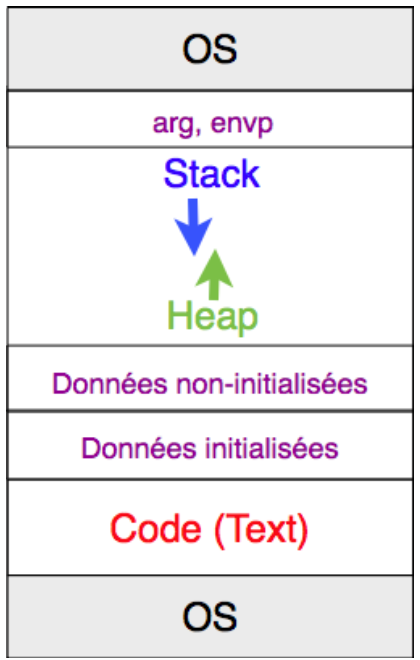
\includegraphics{image-47.png}
\caption{Organisation de la mémoire}
\end{figure}

On a donc 6 segments distincts.

\begin{longtable}[]{@{}
  >{\centering\arraybackslash}p{(\columnwidth - 2\tabcolsep) * \real{0.1590}}
  >{\centering\arraybackslash}p{(\columnwidth - 2\tabcolsep) * \real{0.8410}}@{}}
\toprule\noalign{}
\begin{minipage}[b]{\linewidth}\centering
Zone
\end{minipage} & \begin{minipage}[b]{\linewidth}\centering
Description
\end{minipage} \\
\midrule\noalign{}
\endhead
\bottomrule\noalign{}
\endlastfoot
OS & Réservé à l'OS \\
Segment text & partie la plus basse, en read only. Contient les
instructions à exécuter. Écrire dessus va déclencher un \emph{trap} et
le SE prend le contrôle \\
\emph{Statique}: initialisée & (statique correspond à des données
connues avant l'exécution). Explicitement initialisée ou statique \\
\emph{Statique}: non-initialisée & mise à 0 par le compilateur. \\
Heap & juste après les non-init. Un programme peut y réserver de la
mémoire dessus. On reçoit un pointeur vers le début de la zone.
(\texttt{malloc}) \\
Stack & Démarre vers le haut de l'espace mémoire. Cela stocke les
variables \textbf{locales} et permet l'appel de fonction. (paramètre
d'appel, valeur de retour) et c'est LIFO. \\
Arguments et variables d'environnement & Tout d'au-dessus, on a les
données fournies par le SE en lecture seule. Typiquement les données
qu'on passe quand on lance un programme + variable d'environnement
(\texttt{getenv}, \texttt{unsetenv}, \texttt{setenv}, \ldots). \\
\end{longtable}

Il faut savoir que les variables locales non initialisées \textbf{ne
sont pas mises à 0}. Donc attention au garbage data !

\subsection{Gestion de la mémoire
dynamique}\label{gestion-de-la-muxe9moire-dynamique}

L'allocation de mémoire dynamique est une partie de la librairie
standard. On peut parfois faire des appels systèmes pour étendre la zone
mémoire liée au heap.

\begin{figure}
\centering
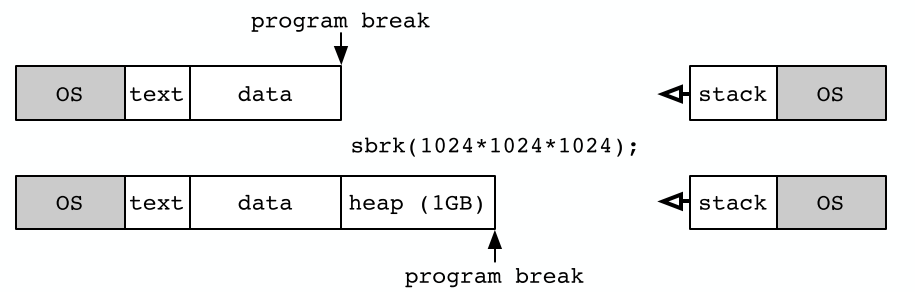
\includegraphics{image-48.png}
\caption{Gestion du heap}
\end{figure}

On voit que \texttt{sbrk} réalise un élargissement de la zone de heap.

\begin{Shaded}
\begin{Highlighting}[]
\PreprocessorTok{\#include }\ImportTok{\textless{}unistd.h\textgreater{}}\PreprocessorTok{ }

\DataTypeTok{int}\NormalTok{ brk}\OperatorTok{(}\DataTypeTok{void} \OperatorTok{*}\NormalTok{addr}\OperatorTok{);}            \CommentTok{// Positionne le programme break a une adresse}
\DataTypeTok{void} \OperatorTok{*}\NormalTok{sbrk}\OperatorTok{(}\DataTypeTok{intptr\_t}\NormalTok{ increment}\OperatorTok{);} \CommentTok{// Décale le programme break et retourne le nouveau program break. }
                                \CommentTok{//(sbrk(0) retourne la valeur actuelle donc)}
\end{Highlighting}
\end{Shaded}

Attention à ne pas trop incrémenter sous peine de cause une erreur.
--\textgreater{} \texttt{ENOMEM} et le processus sera arrêté par le SE.
La limite se trouve via \texttt{ulimit\ -a}.

\subsubsection{Allouer de la mémoire}\label{allouer-de-la-muxe9moire}

On a différentes contraintes:

\begin{itemize}
\tightlist
\item
  Conserver l'information sur les blocs libres et allouées (via
  méta-données)
\item
  méta-données dans le heap
\item
  Trouver le bon endroit pour les mettre
\end{itemize}

\paragraph{Alignement}\label{alignement}

Les données dans la mémoire sont toutes \textbf{alignées}. Souvent sous
un nombre d'octets entiers --\textgreater{} multiple de 2. Sous linux
c'est 16 octets (128bits).

Donc allouer 17 octets va en réalité nous couter 32 octets.

L'utilité principale (comme vu dans le projet) est que les bits de poids
faibles seront toujours à 0. (effectivement \texttt{0b00000000}
--\textgreater{} \texttt{0b00010000} --\textgreater{}
\texttt{0b00100000} --\textgreater{} \ldots). Ainsi, on peut prendre
avantages de ces 4 bits toujours mis à 0 en les utilisant comme des
méta-données.

\paragraph{Objectifs}\label{objectifs}

3 critères pour un bon algorithme de mémoire dynamique:

\begin{enumerate}
\def\labelenumi{\arabic{enumi}.}
\tightlist
\item
  Temps d'exécution faible, stable
\item
  Peu de fragmentation (avoir des trous vides)
\item
  Bonne localité (garder les données proches l'une des autres)
\end{enumerate}

Fragmentation: interne si espace perdu à cause du padding, externe si
manque de place et blocs vides.

\subsubsection{Principe de cache}\label{principe-de-cache}

\begin{figure}
\centering
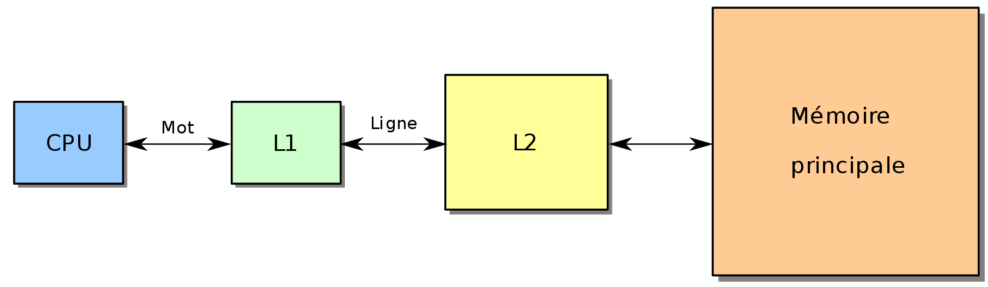
\includegraphics{image-49.png}
\caption{Le cache}
\end{figure}

Pas d'accès à la mémoire cache car trop lente. Au plus elle est rapide
au plus elle coute chère. On a une granularité du cache qui est de 64
octets, cela veut dire qu'on lit à chaque fois 64 octets.

\paragraph{Localité}\label{localituxe9}

Le cache joue sur la localité:

\begin{itemize}
\tightlist
\item
  \emph{Localité Spatiale}: accès à une donné suivie d'accès contiguës.
\item
  \emph{Localité Temporelle}: une donnée récemment lue est souvent dans
  le cache
\end{itemize}

\subsubsection{Implémentation de Notre
Malloc}\label{impluxe9mentation-de-notre-malloc}

On stocke dans 1 bloc de métadonnées la taille de bloc qui est libre + 1
et dans le bit de poids faible le drapeau si c'est alloué ou pas.

C'est pour ça qu'on alloue de minimum 2 comme ça le dernier bit peut
être comme un flag. On peut l'isoler en utilisant des masques
\texttt{c\ \&\ 0x1}.

On peut facilement scinder des blocs en deux etc.

\paragraph{Free}\label{free}

Rien de plus simple, on change le drapeau du bit de poids faible à 0. On
évite de checker si l'utilisateur nous renvoie un bon pointeur car coûte
\(O(n)\).

Mais faire cela va fragmenter notre mémoire, on va généralement
fusionner le nouveau bloc libre avec les blocs libres immédiatement à
gauche et à droite. Mais on a besoin d'une approche \textbf{double
linkedlist} pour ça.

\begin{figure}
\centering
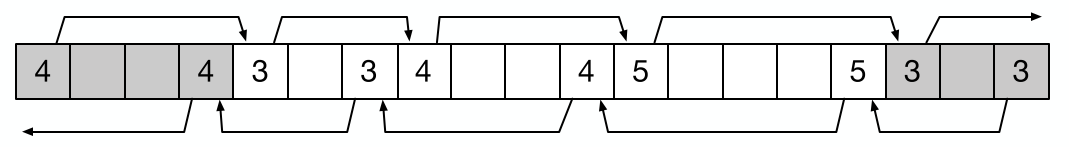
\includegraphics{image-50.png}
\caption{Double LinkedList}
\end{figure}

\paragraph{Politique}\label{politique}

First fit:

\begin{itemize}
\tightlist
\item
  ✅ Rapide car trouve le premier bloc libre
\item
  ❌ Fragmentation
\item
  ❌ Localité faible et devient de pire en pire
\end{itemize}

Next fit (un first fit qui commence au dernier bloc alloué):

\begin{itemize}
\tightlist
\item
  ✅ Rapide
\item
  ❌ Fragmentation de fou furieux
\item
  ✅ Bonne localité
\end{itemize}

Best fit (parcours la liste pour trouver le bloc le plus petit possible
pour notre nouvelle donnée):

\begin{itemize}
\tightlist
\item
  ❌ Lenttttt
\item
  ✅ Fragmentation minime
\item
  ❌ Localité pas ouf
\end{itemize}

\subsubsection{Approche par Liste
Explicite}\label{approche-par-liste-explicite}

On lit les blocs vides entre eux ! Le premier bloc vide sera la taille
de l'ensemble et son second indiquera le prochain bloc vide. On peut
combiner cela à une approche doublement chaînée.

\begin{figure}
\centering
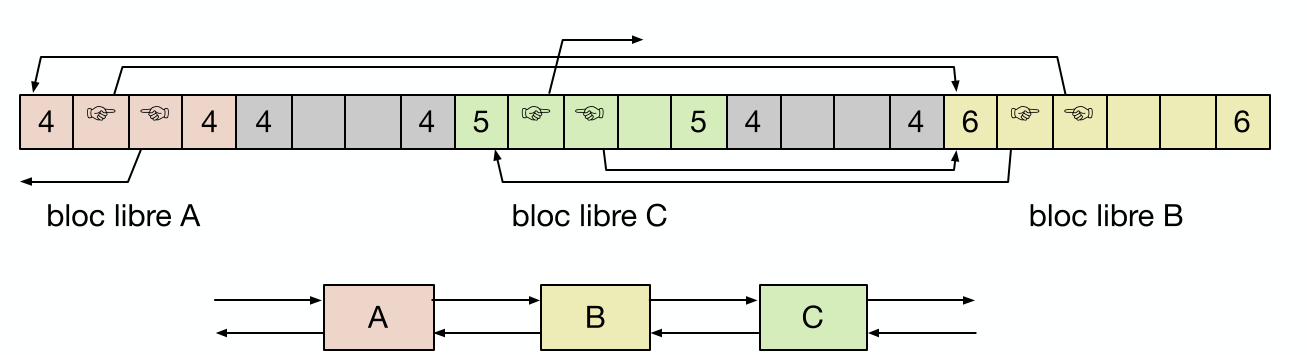
\includegraphics{image-51.png}
\caption{Double LinkedList Explicite}
\end{figure}

On doit donc gérer les insertions et suppressions de blocs. 2 solutions:

\begin{enumerate}
\def\labelenumi{\arabic{enumi}.}
\tightlist
\item
  Insérer en fonction de l'adresse: nous coûte cher car on doit tout
  parcourir mais simple à fusionner
\item
  LIFO: on supprime au bout (facile) mais fusion plus compliquée.
\end{enumerate}

On peut aussi voir une approche différente où on a plusieurs listes en
fonction de la taille de bloc disponible mais ça devient très couteux et
de plus en plus cher.

Tout est une question de compromis comme toujours.
